% 2010 年重庆卷文科第 21 题：双曲线 C（中心 O，右焦点 F）与两条渐近线、直线 l1、l2、MN 的位置图。
% 来源 PDF：普通高考/2010/2010重庆文.pdf，SHA-256 634c8ac529a6ea52305b2909eff8730888048b77d082897394bfda22cb3fe73b。
% 原页：第 2 页（A3 三栏）第 3 栏中部，书页码 580。
% 重绘依据：按原页图形拓扑重绘，坐标取在本图自己的尺度上，并满足题设关系：
%   原点 O(0,0)；x 轴约 -1.5～7.4，y 轴约 -3.2～4.0；
%   双曲线只画右支 x=2√(1+y²)（原页即只画右支，线较粗）；
%   两条渐近线均自 O 向右上方、右下方画出（原页也不画左半段）；
%   取 E(3.61,-1.50) 在右支上，l1 过 M(-1.00,-1.27)，l2 过 N(1.80,0.42)；
%   MN 过 M、N（即 x_E x + 4y_E y = 4），与 y=x/2 交于 G(6.60,3.30)、与 y=-x/2 交于 H(0.61,-0.30)；
%   原页 M、N 为实心圆点，E、G、H 无圆点；E 为 l1、l2 的交点，不在 MN 上。
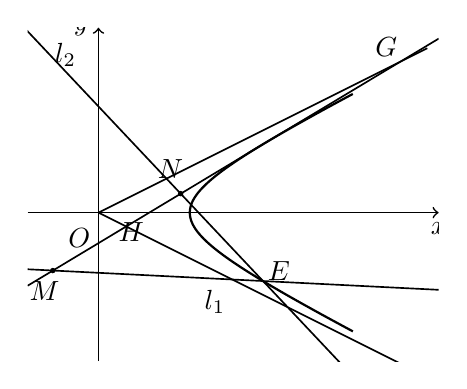
\begin{tikzpicture}[scale=0.58, semithick]
  \coordinate (O) at (0,0);
  \coordinate (M) at (-1.00,-1.268);
  \coordinate (N) at (1.80,0.416);
  \coordinate (E) at (3.606,-1.50);
  \coordinate (G) at (6.60,3.30);
  \coordinate (H) at (0.606,-0.303);

  \clip (-1.55,-3.25) rectangle (7.45,4.05);

  % 坐标轴
  \draw[->] (-1.55,0) -- (7.45,0) node[below] {$x$};
  \draw[->] (0,-3.25) -- (0,4.05) node[left] {$y$};

  % 双曲线右支 x^2/4-y^2=1
  \draw[thick] plot[domain=-2.60:2.60, samples=140, variable=\y]
    ({2*sqrt(1+\y*\y)}, \y);

  % 渐近线 y=±x/2（只画右半）
  \draw (O) -- (7.20,3.60);
  \draw (O) -- (7.20,-3.60);

  % l1（过 M、E）、l2（过 N、E）、MN（过 M、N）
  \draw (-1.55,-1.24) -- (7.45,-1.69);
  \draw (-1.60,4.023) -- (5.40,-3.404);
  \draw (-1.55,-1.60) -- (7.45,3.81);

  % 点 M、N 处实心圆点
  \fill (M) circle (1.7pt);
  \fill (N) circle (1.7pt);

  % 文字（位置照原页）
  \node at (-0.72,3.45) {$l_2$};
  \node at (2.55,-1.95) {$l_1$};
  \node at (-0.42,-0.55) {$O$};
  \node at (-1.18,-1.72) {$M$};
  \node at (1.58,0.95) {$N$};
  \node at (6.30,3.62) {$G$};
  \node at (0.72,-0.42) {$H$};
  \node at (3.95,-1.28) {$E$};
\end{tikzpicture}
